\clearpage
\chapter{Serial communication protocols} \label{Basics_motor_control}

\section{UART (Universal Asynchronous Receiver/Transmitter)}

\begin{figure}[h!]
\centering
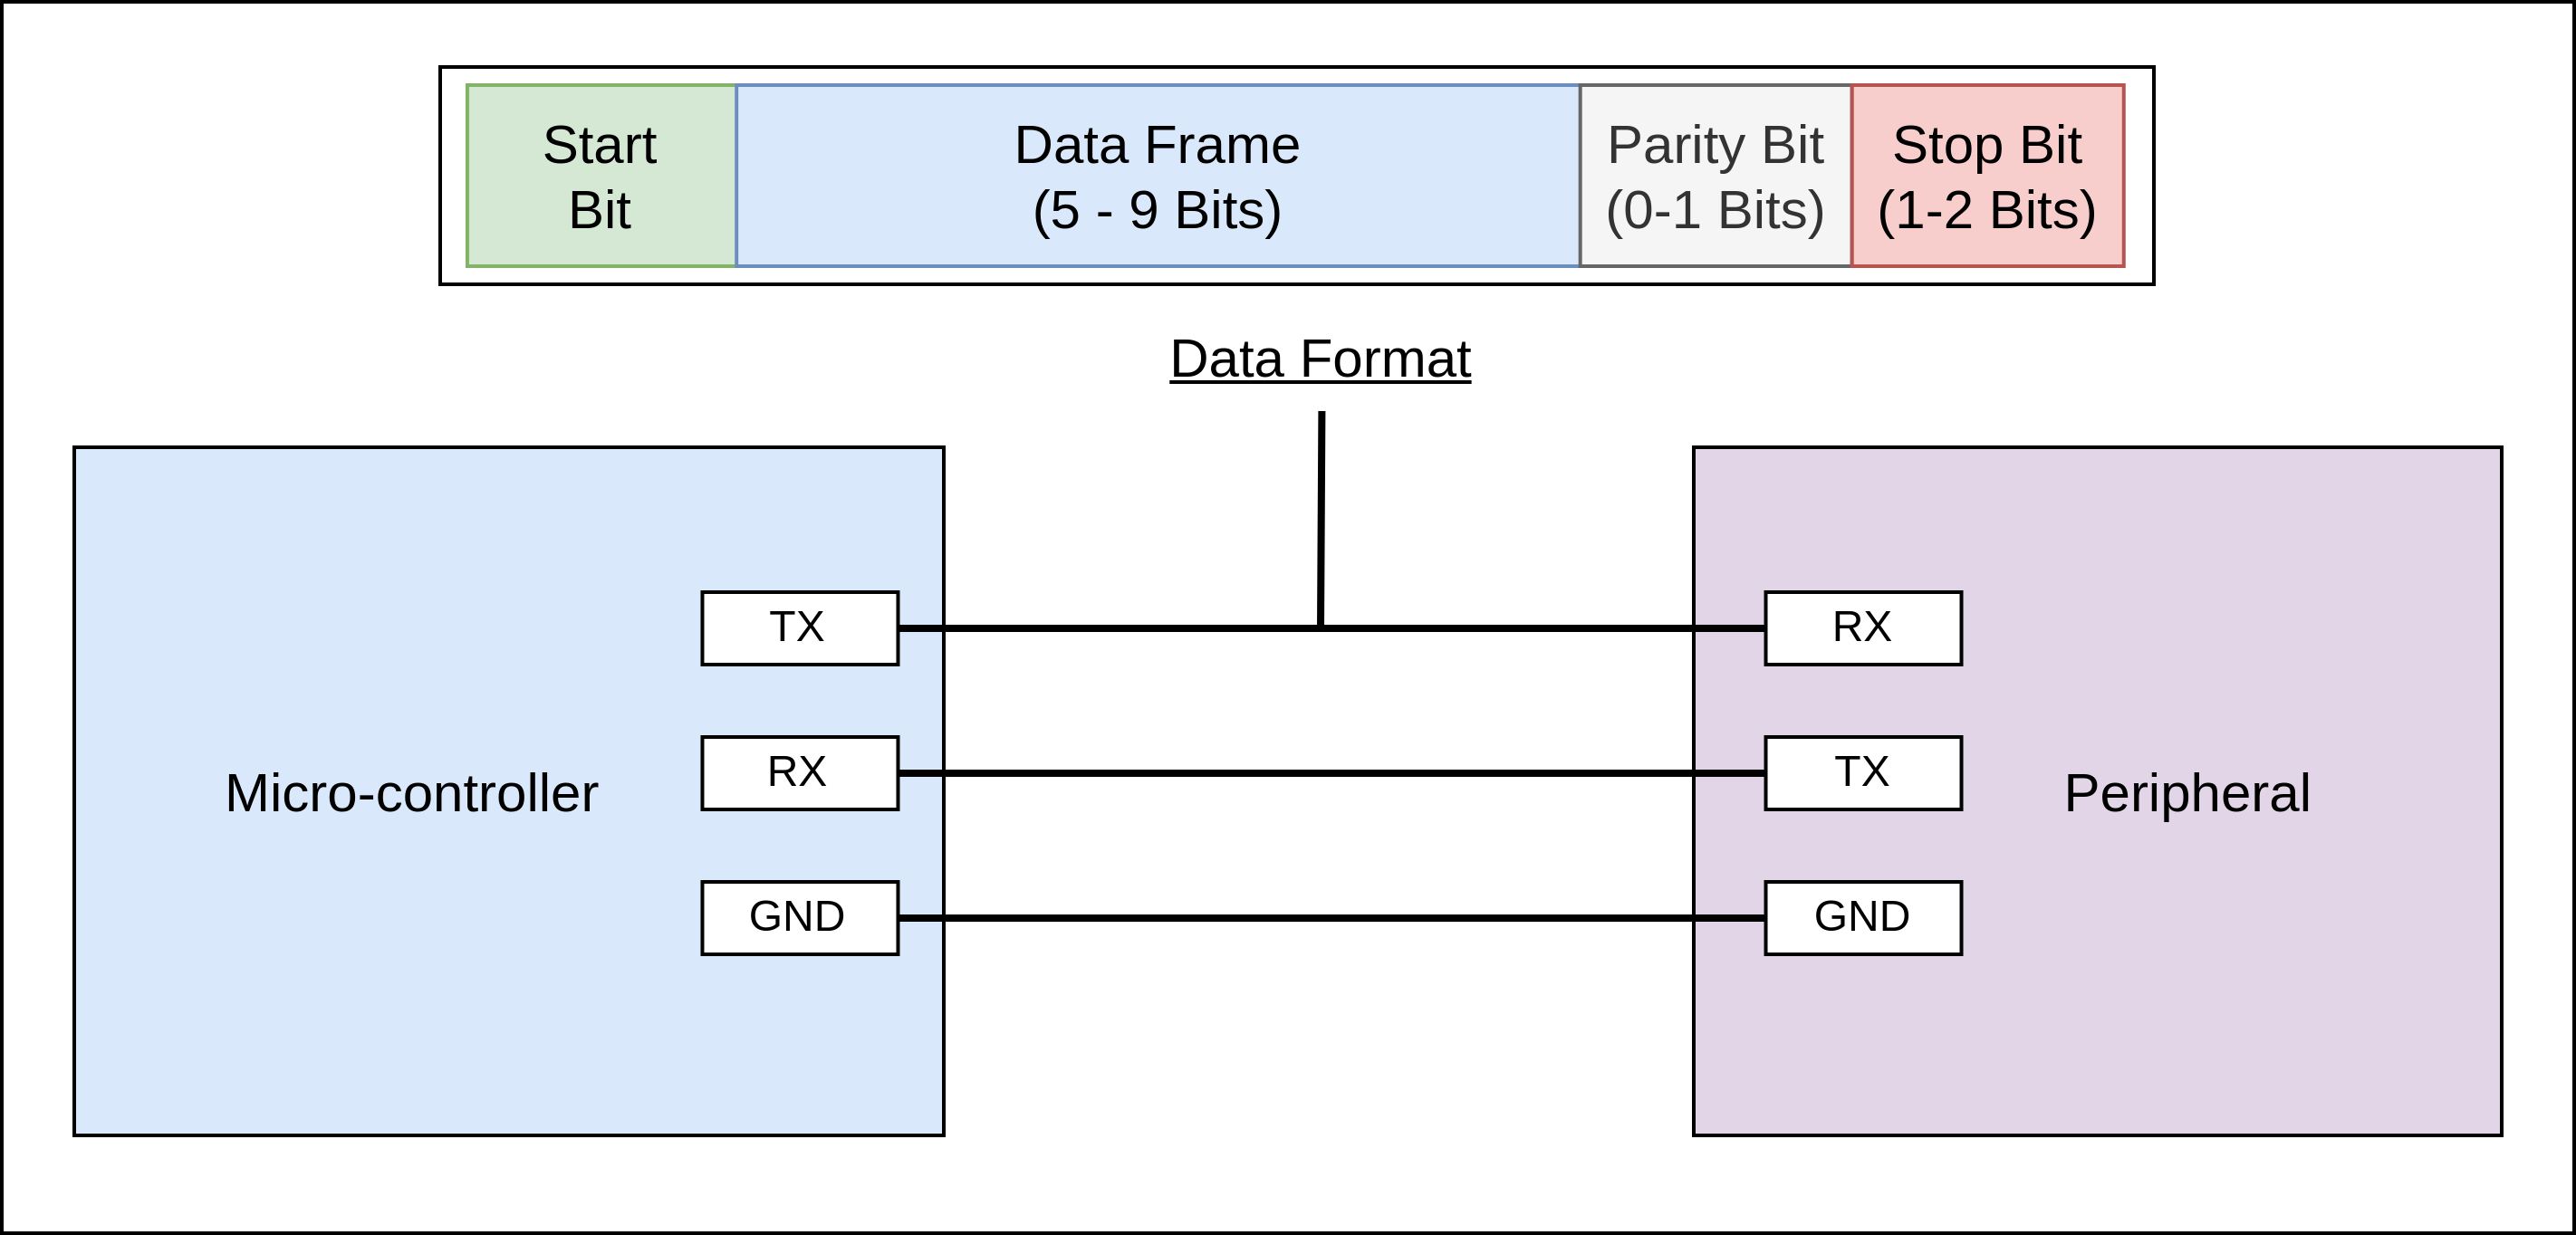
\includegraphics[width=14cm]{./Figures/UART.png}
\caption{Data format and connection between two devices in UART interface}
\label{UART}
\end{figure}

Features of UART interface:
\begin{itemize}
    \item UART is a lower data serial communication protocol. The receiver device should know baud-rate of the transmitter device before actual communication establishment.
    \item UART is simple protocol, it uses start bit, stop bits, parity bit in its base format for data formatting. Parity bit helps in one bit error detection.
    \item Data is transmitted byte by byte. UART does not have clock as it is asynchronous serial communication protocol. It makes use of stop and start bits to synchronise the communication process. Voltages are converted from the 5V to +12V for logic 0 and -12V for logic 1 for long-distance communication. The figure \ref{UART} below shows UART interface between two devices~\cite{Serial_protocols}.  
\end{itemize}

\section{SPI (Serial Peripheral Interface)}
\begin{itemize}
    \begin{figure}[h!]
    \centering
    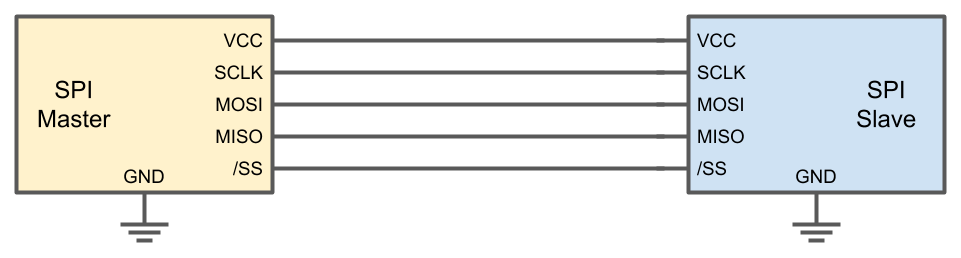
\includegraphics[width=11cm]{./Figures/SPI_single_slave.png}
    \caption{SPI point-to-point connections}
    \label{SPI_single_slave}
    \end{figure}
    \item SPI is a serial protocol consisting of 4 signal lines:
    \begin{itemize}
        \item \textbf{SCLK:} The clock signal is sent from the master to the slaves; It helps in synchronization of other SPI signals.
        \item \textbf{SS:} Slave select signal is used to select the slave device to which the data is communicated by the master.
        \item \textbf{MOSI:} It is a data line from the master to the slaves. It stands for Master Out-Slave In.
        \item \textbf{MISO:} It is a data line from the slaves to the master. It stands for Master In-Slave Out.
    \end{itemize}
    \item There are typically two SPI bus topologies:
    \begin{itemize}
        \item \textbf{Point-to-Point topology:} SPI Master is connected to a single slave as shown in Figure \ref{SPI_single_slave}.
        \item \textbf{Point-to-Multipoint topology:} SPI Master is connected to multiple slaves as shown in Figure \ref{SPI_multi_slave}~\cite{Serial_protocols}.
    \end{itemize}
    \begin{figure}[h!]
    \centering
    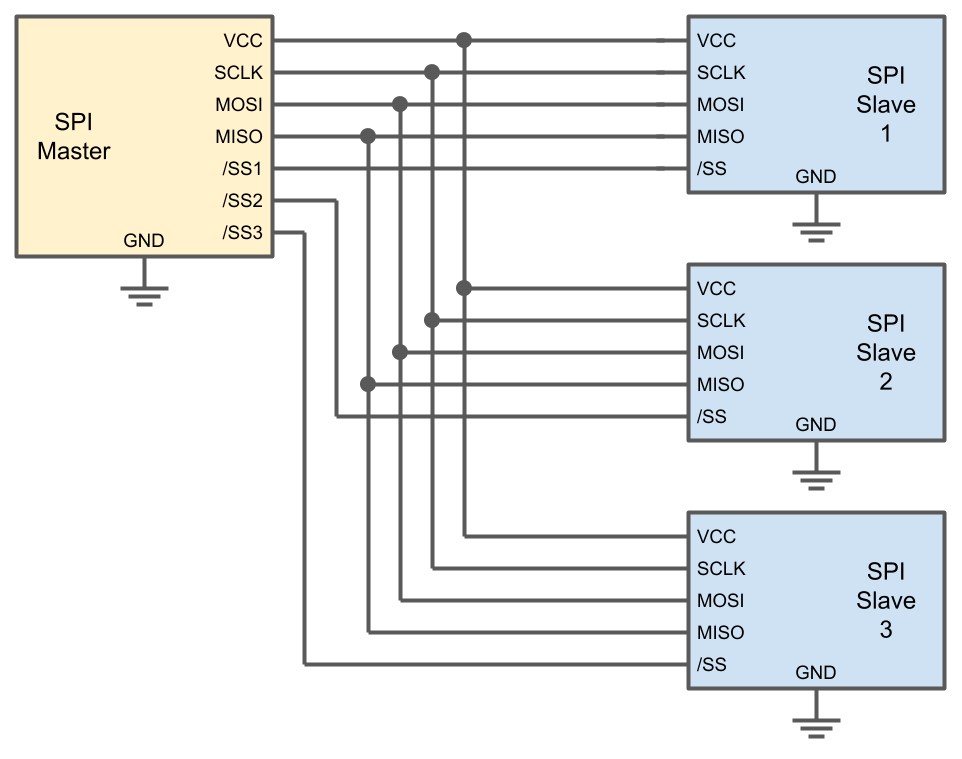
\includegraphics[width=11cm]{./Figures/SPI_multi_slave.png}
    \caption{SPI connections for 3 slave devices}
    \label{SPI_multi_slave}
    \end{figure}
\end{itemize}

\newpage
\section{I2C Protocol}

\begin{figure}[h!]
\centering
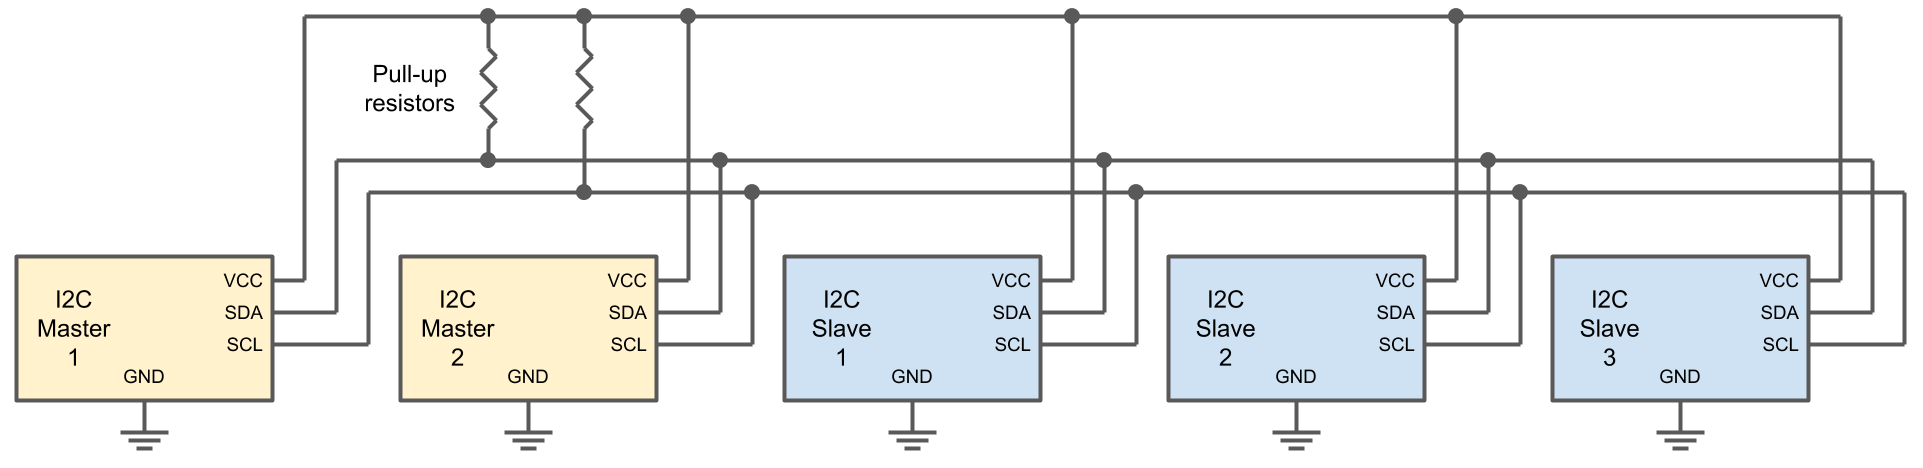
\includegraphics[width=\columnwidth]{./Figures/I2C_multi_master.png}
\caption{I2C connections for multiple master and multiple slave devices}
\label{I2C_multi_master}
\end{figure}

Features:
\begin{itemize}
    \item Unlike SPI, I2C is a 2-wire communication protocol which is commonly used for connection of low-speed devices like I/O interfaces, ADC and DAC, EEPROMs and other peripherals in embedded systems.
    \item \textbf{SCL (Serial Clock)} carries the clock signal.
    \item \textbf{SDA (Serial Data)} allows master and slave devices connected to the bus to send/receive data. 
    \item I2C allows multiple slave connections to a single master device, or  multiple masters controlling one or more slaves (Figure \ref{I2C_multi_master})~\cite{Serial_protocols}.
\end{itemize}
